%%%%%%%%%%%%%%%%%%%%%%%%%%%%%%%%%%%%%%%%%
% Masters/Doctoral Thesis 
% LaTeX Template
% Version 2.5 (27/8/17)
%
% This template was downloaded from:
% http://www.LaTeXTemplates.com
%
% Version 2.x major modifications by:
% Vel (vel@latextemplates.com)
%
% This template is based on a template by:
% Steve Gunn (http://users.ecs.soton.ac.uk/srg/softwaretools/document/templates/)
% Sunil Patel (http://www.sunilpatel.co.uk/thesis-template/)
%
% Template license:
% CC BY-NC-SA 3.0 (http://creativecommons.org/licenses/by-nc-sa/3.0/)
%
%%%%%%%%%%%%%%%%%%%%%%%%%%%%%%%%%%%%%%%%%

%----------------------------------------------------------------------------------------
%	PACKAGES AND OTHER DOCUMENT CONFIGURATIONS
%----------------------------------------------------------------------------------------

\documentclass[
11pt, % The default document font size, options: 10pt, 11pt, 12pt
%oneside, % Two side (alternating margins) for binding by default, uncomment to switch to one side
english, % ngerman for German
singlespacing, % Single line spacing, alternatives: onehalfspacing or doublespacing
%draft, % Uncomment to enable draft mode (no pictures, no links, overfull hboxes indicated)
%nolistspacing, % If the document is onehalfspacing or doublespacing, uncomment this to set spacing in lists to single
%liststotoc, % Uncomment to add the list of figures/tables/etc to the table of contents
%toctotoc, % Uncomment to add the main table of contents to the table of contents
%parskip, % Uncomment to add space between paragraphs
%nohyperref, % Uncomment to not load the hyperref package
headsepline, % Uncomment to get a line under the header
%chapterinoneline, % Uncomment to place the chapter title next to the number on one line
%consistentlayout, % Uncomment to change the layout of the declaration, abstract and acknowledgements pages to match the default layout
openany
]{MastersDoctoralThesis} % The class file specifying the document structure

\usepackage[utf8]{inputenc} % Required for inputting international characters
\usepackage[T1]{fontenc} % Output font encoding for international characters

\usepackage{mathpazo} % Use the Palatino font by default

\usepackage[
backend=bibtex,
style=numeric,
% citestyle=authoryear,
natbib=true
]{biblatex} % Use the bibtex backend with the authoryear citation style (which resembles APA)

\addbibresource{thesis.bib} % The filename of the bibliography

\usepackage[autostyle=true]{csquotes} % Required to generate language-dependent quotes in the bibliography

\usepackage{bera}% optional: just to have a nice mono-spaced font
\usepackage{listings}
\usepackage{xcolor}

\usepackage{graphicx}
\usepackage{hyperref}
\urlstyle{same}

\definecolor{eclipseStrings}{RGB}{42,0.0,255}
\definecolor{eclipseKeywords}{RGB}{127,0,85}
\definecolor{background}{HTML}{EEEEEE}
\colorlet{numb}{magenta!60!black}

\lstdefinelanguage{json}{
    basicstyle=\small\ttfamily,
    commentstyle=\color{eclipseStrings}, % style of comment
    stringstyle=\color{eclipseKeywords}, % style of strings
    numbers=left,
    numberstyle=\scriptsize,
    stepnumber=1,
    numbersep=8pt,
    showstringspaces=false,
    breaklines=true,
    frame=lines,
    backgroundcolor=\color{background}, %only if you like
    string=[s]{"}{"},
    comment=[l]{:\ "},
    morecomment=[l]{:"},
    literate=
        *{0}{{{\color{numb}0}}}{1}
         {1}{{{\color{numb}1}}}{1}
         {2}{{{\color{numb}2}}}{1}
         {3}{{{\color{numb}3}}}{1}
         {4}{{{\color{numb}4}}}{1}
         {5}{{{\color{numb}5}}}{1}
         {6}{{{\color{numb}6}}}{1}
         {7}{{{\color{numb}7}}}{1}
         {8}{{{\color{numb}8}}}{1}
         {9}{{{\color{numb}9}}}{1}
}

%----------------------------------------------------------------------------------------
%	MARGIN SETTINGS
%----------------------------------------------------------------------------------------

\geometry{
	paper=a4paper, % Change to letterpaper for US letter
	inner=2.5cm, % Inner margin
	outer=3.8cm, % Outer margin
	bindingoffset=.5cm, % Binding offset
	top=1.5cm, % Top margin
	bottom=1.5cm, % Bottom margin
	%showframe, % Uncomment to show how the type block is set on the page
}

%----------------------------------------------------------------------------------------
%	THESIS INFORMATION
%----------------------------------------------------------------------------------------

\thesistitle{Image Recommendation for Wikipedia Articles} % Your thesis title, this is used in the title and abstract, print it elsewhere with \ttitle
\supervisor{Miriam \textsc{Redi}} % Your supervisor's name, this is used in the title page, print it elsewhere with \supname
\examiner{} % Your examiner's name, this is not currently used anywhere in the template, print it elsewhere with \examname
\degree{Master of Science} % Your degree name, this is used in the title page and abstract, print it elsewhere with \degreename
\author{Oleh \textsc{Onyshchak}} % Your name, this is used in the title page and abstract, print it elsewhere with \authorname
\addresses{} % Your address, this is not currently used anywhere in the template, print it elsewhere with \addressname

\subject{Data Science} % Your subject area, this is not currently used anywhere in the template, print it elsewhere with \subjectname
\keywords{} % Keywords for your thesis, this is not currently used anywhere in the template, print it elsewhere with \keywordnames
\university{\href{http://www.ucu.edu.ua}{Ukrainian Catholic University}} % Your university's name and URL, this is used in the title page and abstract, print it elsewhere with \univname
\department{\href{http://department.university.com}{Faculty of Applied Sciences}} % Your department's name and URL, this is used in the title page and abstract, print it elsewhere with \deptname
\group{\href{http://researchgroup.university.com}{Department of Computer Sciences}} % Your research group's name and URL, this is used in the title page, print it elsewhere with \groupname
\faculty{\href{http://faculty.university.com}{}} % Your faculty's name and URL, this is used in the title page and abstract, print it elsewhere with \facname

\AtBeginDocument{
\hypersetup{pdftitle=\ttitle} % Set the PDF's title to your title
\hypersetup{pdfauthor=\authorname} % Set the PDF's author to your name
\hypersetup{pdfkeywords=\keywordnames} % Set the PDF's keywords to your keywords
}

\begin{document}
\frontmatter % Use roman page numbering style (i, ii, iii, iv...) for the pre-content pages

\pagestyle{plain} % Default to the plain heading style until the thesis style is called for the body content

%----------------------------------------------------------------------------------------
%	TITLE PAGE
%----------------------------------------------------------------------------------------

\begin{titlepage}
\begin{center}

\vspace*{.06\textheight}
{\scshape\LARGE \univname\par}\vspace{1.5cm} % University name
\textsc{\Large Master Thesis}\\[0.5cm] % Thesis type

\HRule \\[0.4cm] % Horizontal line
{\huge \bfseries \ttitle\par}\vspace{0.4cm} % Thesis title
\HRule \\[1.5cm] % Horizontal line
 
\begin{minipage}[t]{0.4\textwidth}
\begin{flushleft} \large
\emph{Author:}\\
\href{http://www.johnsmith.com}{\authorname} % Author name - remove the \href bracket to remove the link
\end{flushleft}
\end{minipage}
\begin{minipage}[t]{0.4\textwidth}
\begin{flushright} \large
\emph{Supervisor:} \\
\href{http://www.jamessmith.com}{\supname} % Supervisor name - remove the \href bracket to remove the link  
\end{flushright}
\end{minipage}\\[3cm]
 
\vfill

\large \textit{A thesis submitted in fulfillment of the requirements\\ for the degree of \degreename}\\[0.3cm] % University requirement text
\textit{in the}\\[0.4cm]
\groupname\\\deptname\\[1cm] % Research group name and department name
 
\vfill

\includegraphics[height=5cm]{UCU-Apps.png} % University/department logo - uncomment to place it

\vfill
{\large Lviv 2020}\\[4cm] % Date
 
\vfill
\end{center}
\end{titlepage}

%----------------------------------------------------------------------------------------
%	DECLARATION PAGE
%----------------------------------------------------------------------------------------

\begin{declaration}
\addchaptertocentry{\authorshipname} % Add the declaration to the table of contents
\noindent I, \authorname, declare that this thesis titled, \enquote{\ttitle} and the work presented in it are my own. I confirm that:

\begin{itemize} 
\item This work was done wholly or mainly while in candidature for a research degree at this University.
\item Where any part of this thesis has previously been submitted for a degree or any other qualification at this University or any other institution, this has been clearly stated.
\item Where I have consulted the published work of others, this is always clearly attributed.
\item Where I have quoted from the work of others, the source is always given. With the exception of such quotations, this thesis is entirely my own work.
\item I have acknowledged all main sources of help.
\item Where the thesis is based on work done by myself jointly with others, I have made clear exactly what was done by others and what I have contributed myself.\\
\end{itemize}
 
\noindent Signed:\\
\rule[0.5em]{25em}{0.5pt} % This prints a line for the signature
 
\noindent Date:\\
\rule[0.5em]{25em}{0.5pt} % This prints a line to write the date
\end{declaration}

\cleardoublepage

%----------------------------------------------------------------------------------------
%	QUOTATION PAGE
%----------------------------------------------------------------------------------------

\vspace*{0.2\textheight}

\noindent\enquote{\itshape Thanks to my solid academic training, today I can write hundreds of words on virtually any topic without possessing a shred of information, which is how I got a good job in journalism.}\bigbreak

\hfill Dave Barry

%----------------------------------------------------------------------------------------
%	ABSTRACT PAGE
%----------------------------------------------------------------------------------------

\begin{abstract}
\addchaptertocentry{\abstractname} % Add the abstract to the table of contents
Multimodal learning, which is simultaneous learning from different data sources such as audio, text, images; is a rapidly emerging field of Machine Learning. It is also considered to be learning on the next level of abstraction, which will allow us to tackle more complicated problems such as creating cartoons from a plot or speech recognition based on lips movement. 

In this paper, we propose to research whether state-of-the-art techniques of multimodal learning, will solve the problem of recommending the most relevant images for a Wikipedia article. In other words, we need to create a shared text-image representation of an abstract notion which paper describes, so that having only a text description machine would "understand" which images would visualize the same notion accurately. 
\end{abstract}

%----------------------------------------------------------------------------------------
%	ACKNOWLEDGEMENTS
%----------------------------------------------------------------------------------------

\begin{acknowledgements}
\addchaptertocentry{\acknowledgementname} % Add the acknowledgements to the table of contents
The acknowledgments and the people to thank go here, don't forget to include your project advisor\ldots
\end{acknowledgements}

%----------------------------------------------------------------------------------------
%	LIST OF CONTENTS/FIGURES/TABLES PAGES
%----------------------------------------------------------------------------------------

\tableofcontents % Prints the main table of contents

\listoffigures % Prints the list of figures

\listoftables % Prints the list of tables

%----------------------------------------------------------------------------------------
%	ABBREVIATIONS
%----------------------------------------------------------------------------------------

\begin{abbreviations}{ll} % Include a list of abbreviations (a table of two columns)

\textbf{LAH} & \textbf{L}ist \textbf{A}bbreviations \textbf{H}ere\\
\textbf{WSF} & \textbf{W}hat (it) \textbf{S}tands \textbf{F}or\\

\end{abbreviations}

%----------------------------------------------------------------------------------------
%	PHYSICAL CONSTANTS/OTHER DEFINITIONS
%----------------------------------------------------------------------------------------

\begin{constants}{lr@{${}={}$}l} % The list of physical constants is a three column table

% The \SI{}{} command is provided by the siunitx package, see its documentation for instructions on how to use it

Speed of Light & $c_{0}$ & \SI{2.99792458e8}{\meter\per\second} (exact)\\
%Constant Name & $Symbol$ & $Constant Value$ with units\\

\end{constants}

%----------------------------------------------------------------------------------------
%	SYMBOLS
%----------------------------------------------------------------------------------------

\begin{symbols}{lll} % Include a list of Symbols (a three column table)

$a$ & distance & \si{\meter} \\
$P$ & power & \si{\watt} (\si{\joule\per\second}) \\
%Symbol & Name & Unit \\

\addlinespace % Gap to separate the Roman symbols from the Greek

$\omega$ & angular frequency & \si{\radian} \\

\end{symbols}

%----------------------------------------------------------------------------------------
%	DEDICATION
%----------------------------------------------------------------------------------------

\dedicatory{For/Dedicated to/To my\ldots} 

%----------------------------------------------------------------------------------------
%	THESIS CONTENT - CHAPTERS
%----------------------------------------------------------------------------------------

\mainmatter % Begin numeric (1,2,3...) page numbering

\pagestyle{thesis} % Return the page headers back to the "thesis" style

% Include the chapters of the thesis as separate files from the Chapters folder
% Uncomment the lines as you write the chapters

\chapter{Introduction}
\section{Domain Overview}

Every day we perceive the world around us through multiple cognitive feelings such as sight, smell, hearing, touch, taste. Moreover, our ability to consolidate all the information from different sources into one complete picture helps us comprehensively understand the world.

With a trend to digitizing in the last few decades, more and more information is recorded in different kids of medial such as audio, image, video, text, and 3D modeling. That also created new challenges of efficiently processing a significant amount of recorded information, where we already have significant achievements. However, every type of digital storage only captures some subset of available information. For example, image only captures visual appearance, while  audio - the sound, just as our eyes and ears do. Thus all scientific progress in processing some data carrier is bounded by limitation of what that medium can capture. In other words, to digitally create a notion of a dog, we cannot only have a visual representation. Just as humans, we need to combine all the information streams, which describe the same entity from different perspectives, into one comprehensive representation.

That is the motivation for multimodal representation learning, which aims to combine different types of data into a complete representation of a real-world entity. In that context, the word "modality" refers to a particular way of encoding information. Thus a problem in the domain of e.g., image processing is called unimodal, while a problem in the domain of multiple information encodings e.g., image to caption generation, is called multimodal since it works with both: image and text modalities \cite{ref_survey} 

By having a complete representation of an entity, which was created via multimodal data that captures complementary/supplementary information subsets of an object, we have more comprehensive computational "understanding" of that entity. That will help us to increase the precision of existing data science applications and also extend its limits to more abstract problems such as not only identifying the objects on an image but understanding its value. For example\cite{ref_survey}, early researches on speech recognition showed that by involving visual modality of lips movement on top of sound modality, we get extra information which allows us to increase the quality of voice recognition task, just as it does for humans\cite{ref_human_voice_recognition}

In this project, we are going to research possible approaches for the "Image Recommendation for Wikipedia Articles" problem, which is also part of multimodal representation learning domain. That is, based on the article's text information, we need to recommend images describing the same notion. In other words, we need to create a high-level representation of some entity, described by both text and images. So that later one we can "understand" which image representation of the notion is the best suited for a given text description.

In scope of this project, we are going to explore state-of-the-art techniques of multimodal representation learning and whether they can be applied to solve this problem. We believe this project will be valuable from both a research and an application perspectives.

This report is an official Project Proposal of Master's Thesis, which will formally define the problem, provide rigor overview of state-of-the-art approaches in problem's domain, specify goals of the project, suggest a solution approach and provide a time plan of the thesis.

\section{Problem Motivation}
Wikipedia is the biggest collection of human knowledge containing more than 35 million pages and having nearly 9 billion views per month\footnote{\url{https://stats.wikimedia.org/v2/##/en.wikipedia.org}} And it continually growing, having more than 500 new pages per day\footnote{\url{https://en.wikipedia.org/wiki/Wikipedia:Statistics}}, and all of that only in its English version.

As a part of 2030 strategy, one of the key goals is to break down any barriers for accessing free information\footnote{\url{https://meta.wikimedia.org/wiki/Strategy/Wikimedia_movement/2017/Direction}}. By researching possibilities to automatically recommend images for Wikipedia editors, it will help to get better media enrichment of articles, which in turn will make information easier and faster to comprehend\cite{ref_image_attention}. Also, it would be helpful as automation of time-consuming task to search for and add a proper article visualization. 

In addition to motivation of making Wikipedia better, this work might present some useful insights to development of multimodal learning field. Since this is a 1) purely real-world problem, which might give us interesting insights of how to apply and adjust current academia progress, and also 2) we have a more complicated problem setting of one large article corresponding to a multiple images, instead of more simplified one-to-one correspondas of images and its tags/descriptive sentences.


\section{Problem Formulation}
We are going to research how state-of-the-art multimodal learning techniques performs on a task of recommending images for Wikipedia articles. In other words, having a text with wiki formatting, we need to rank images from Wikimedia Commons database\cite{ref_wiki_commons} by relevance.

\endinput
\chapter{Related Work}
\section{Overview}
While during the last decades there was much progress in a field of unimodal representation, research in multimodal learning was limited by simple concatenation of unimodal features\cite{ref_survey_2015}. However, during recent years, the scientific landscape in this domain has been rapidly evolving\cite{ref_survey_baltrusaitis}. One of the triggers for it was the success of deep learning models, which have a powerful representation ability with multiple levels of abstractions. Thus they were also incorporated in multimodal learning. As Guo et al. suggested\cite{ref_survey}, we can divide all the multimodal learning approaches into three categories 1) joint representation, which aims to integrate modality-specific features into some common space 2) coordinated representation, which aims to preserve modality-specific features, while introducing a space to measure multimodal similarities  3) intermediate representation, which aims to encode features of one modal to some intermediate space, from where we later generate features of another modal.

In this chapter, we will cover available techniques to extract features from text and image modalities, overview available solutions in each type of multimodal learning, and then summarise their applicability for our problem.

\section{Unimodal Representation}
\subsection{Image}
The most popular model used in feature extraction from images are different types of Convolutional Neural Network(CNN), such as AlexNet\cite{ref_AlexNet}, VGGNet\cite{ref_VGGNet} and ResNet\cite{ref_ResNet}. When working with big datasets, it is preferable to use pre-trained version of chosen CNN. This field has tremendous development in recent years, and thus currently we already have well-defined solution for most problems.

\subsection{Text}
A popular way to extract features from the text is to encode it to vector, as is done in word2vec\cite{ref_word2vec} or Glove\cite{ref_glove} algorithms. They map words into one-hot encoded vector space of language vocabulary. Although, the common problem with those approaches is when some words are not present in vocabulary or out-of-vocabulary error. However, there are also a variety of solutions to this problem, such as character embeddings\cite{ref_char_embeddings}. 

An alternative and more powerful tool for dealing with text is recurrent neural network(RNN)\cite{ref_rnn}, which is more context-aware and can make better encoding of the n-th word, knowing what was already in a sentence. One of the most successful realizations of RNN is long short-term memory(LSTM)\cite{ref_lstm}.

\begin{figure}
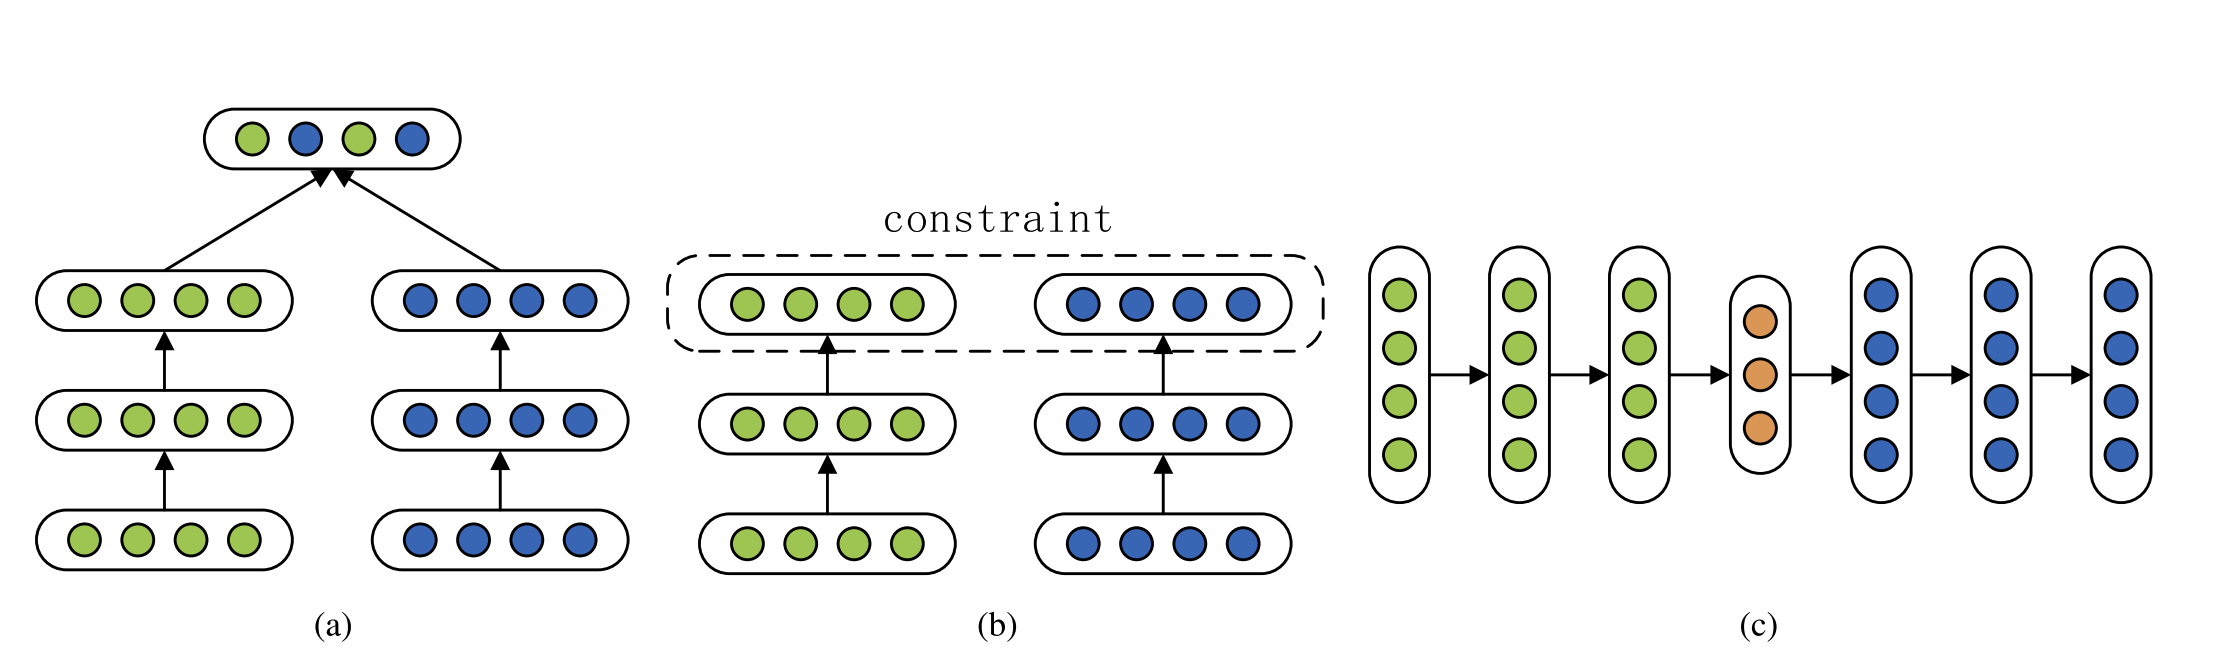
\includegraphics[width=\textwidth]{Resources/multimodal_learning_types.png}
\caption{Three types of frameworks about deep multimodal representation. (a) Joint representation aims to learn a shared semantic subspace.(b) Coordinated representation framework learns separated but coordinated representations for each modality under some constraints.
(c) intermediate representation framework translates one modality into another and keep their semantics consistent.\cite{ref_survey}} \label{fig1}
\end{figure}

\section{Joint Representation}
The main idea of joint representation is to integrate multimodal features into a single input, which we then process as some artificial unimodal input with well-known machine learning techniques. More formally, it aims to project unimodal representations into a shared semantic subspace, where the multimodal features can be fused\cite{ref_survey_baltrusaitis},  as shown in Figure \ref{fig1}(a). Up until recently, that was the primary technique in multimodal learning, where shared features were fused by concatenating them together. However, now,  the most popular choice is to use a distinct hidden layer, where modality-specific features will be combined into a single output vector.

This approach was historically the first one and is still commonly applicable in video classification\cite{ref_video_class}, event detection\cite{ref_event_detection} and visual question answering\cite{ref_visual_question_answ}. However, its main disadvantage is neglecting the fact that different modalities have not only supplementary information, that is which show the same notion from different perspectives, but also complementary information, where one modality captures the information which another cannot. For example, lips movement and audio of a speech are mostly supplementary sources, while images of some bird and audio of it singing are mostly supplementary sources. Because of that, much information gets lost in that shared space. 
% TODO: explain why in examples above one is supplementary and another complemetary

Although it has advantages of being a simple method and producing modality-invariant common space of features, it cannot be used to infer the separated representations for each modality\cite{ref_survey}. Thus methods from this category are not applicable to our problem

\section{Intermediate Representation}
Intermediate Representation models aim to encode features of one modality to some intermediate space, from which later features of another modality can be generated(or decoded), as shown on Figure \ref{fig1}(c). To prevent the intermediate space from being related only to a source modality, during encoder-decoder training we maximize, e.g., the likelihood of target sentence given source image, so that error function employs the error of decoding. Subsequently, the generated intermediate representation tends to capture the shared semantics from both modalities\cite{ref_survey}. 

Some interesting application of that model was proposed by Mor et al.\cite{ref_music_decoder}, where algorithm encodes a musical track into intermediate space, which then will be decoded by multiple decoders into a space of some specific instrument. In other words, encoder extracts instrument-invariant generic musical features, which then each decoder transforms into features of its target instrument.

The general advantage of such approach is that it is one of the best ways to generate new features in a target domain. Thus this technique is used in Image Caption\cite{ref_image_caption}, Video Description\cite{ref_video_description}, and Text to Image\cite{ref_text2image} generations. The disadvantages of that model are that 1) it can only encode one modality, 2) complexity of designing a feature generator should be taken into account\cite{ref_survey} and 3) intermediate space also extracts only shared subspace from two modalities. Moreover, because we need to query existing information rather than generate one, those methods are also not suitable for our problem solution.

\section{Coordinated Representation}
The last type of multimodal learning is a coordinated representation. Instead of learning from a joint representation, it learns from modal-specific representations separately but with a shared constraint, which is some loss function identifying cross-modal similarity/correlation. Since different modalities hold unique information about an object, that approach operates with all available knowledge. A visual explanation can be seen in Figure \ref{fig1}(b). Regarding constraint function, a commonly used option is cross-modal similarity functions, where learning objective is to preserve both inter-modality and intra-modality similarity structure. In other words, it would force cross-modal distance for elements with the same semantics be as small as possible, while with dissimilar - as big as possible. 

% TODO: specify what specifically function S can be and how it works. Note
% about copy-paste from here into solution approach
The cross-modal ranking is a widely used constrain, where the loss function is defined in the following way
\begin{equation} \label{eq_rank_loss}
\sum_i \sum_{t^-} max(0, \alpha - S(i, t) + S(i, t^-)) + \sum_t \sum_{i^-} max(0, \alpha - S(t, i) + S(t, i^-))
\end{equation}
where (i,t) is a matching image-text pair, $\alpha$ is margin, S is a similarity function, $i^-$ is mismatching pair to $t$ and vise versa. Frome et al.\cite{ref_devise} used a combination of dot-product similarity and margin rank loss to learn a visual-semantic embedding model(DeViSE) for visual recognition\cite{ref_survey}. DeViSE trains deep networks for both image and text features, and then adjust features based on above mentioned ranked loss, though in more simplified form.

Alternatively to cross-modal ranking, another widely used constraint is Euclid distance, which is also used for ensuring that similarity structure for both intra-modality and inter-modality is preserved. That is, for inter-modality, we map text and image features into low-dimensional space, where we can calculate the distance between feature vectors. The idea here is to ensure that inter-modality features of the same semantics are as close as possible\cite{ref_pan}. While for intra-modality, we want to preserve the similarity between neighborhood items, that is:
\begin{equation} \label{eq_eucl_loss}
d(m_i, m_j) + m < d(m_i, m_k), \forall m_j \in N(m_i), \forall m_k \notin N(m_i)
\end{equation}
where $m$ is data point of any modality, $m_i$ point of interest, N(m) - denotes neighborhood of m\cite{ref_wang}.
% TODO: what is m specifically in a formula? Correct it!

Besides the classical coordinated representation approach, there is a simplified version where instead of mapping both text and visual features into common space, we only map text features into visual space\cite{ref_w2vv}. In this case, we would use constant visual features, e.g. last hidden fully-connected layer of ResNet-152 pretrained on ResNet dataset\cite{ref_ResNet}. Thus we will benefit from significantly faster training time since we will only need to train one neural network for mapping text features into visual space of features. Although, the benefit comes with a cost of precision loss since we loose information specific to text modality.

So, Coordinated Representation preserves all modality-specific information. It also explicitly compares features from different modalities, thus having data from one, we can identify the closest data point from another modality. Because of those properties, it is used for cross-modal retrieval\cite{ref_wang}, retrieval-based visual description\cite{ref_socher}, and transfer knowledge across
\newline
modalities\cite{ref_pan}. Thus it can be applied for our problem of Image Recommendation for articles, and we will proceed with those methods.

\begin{figure}
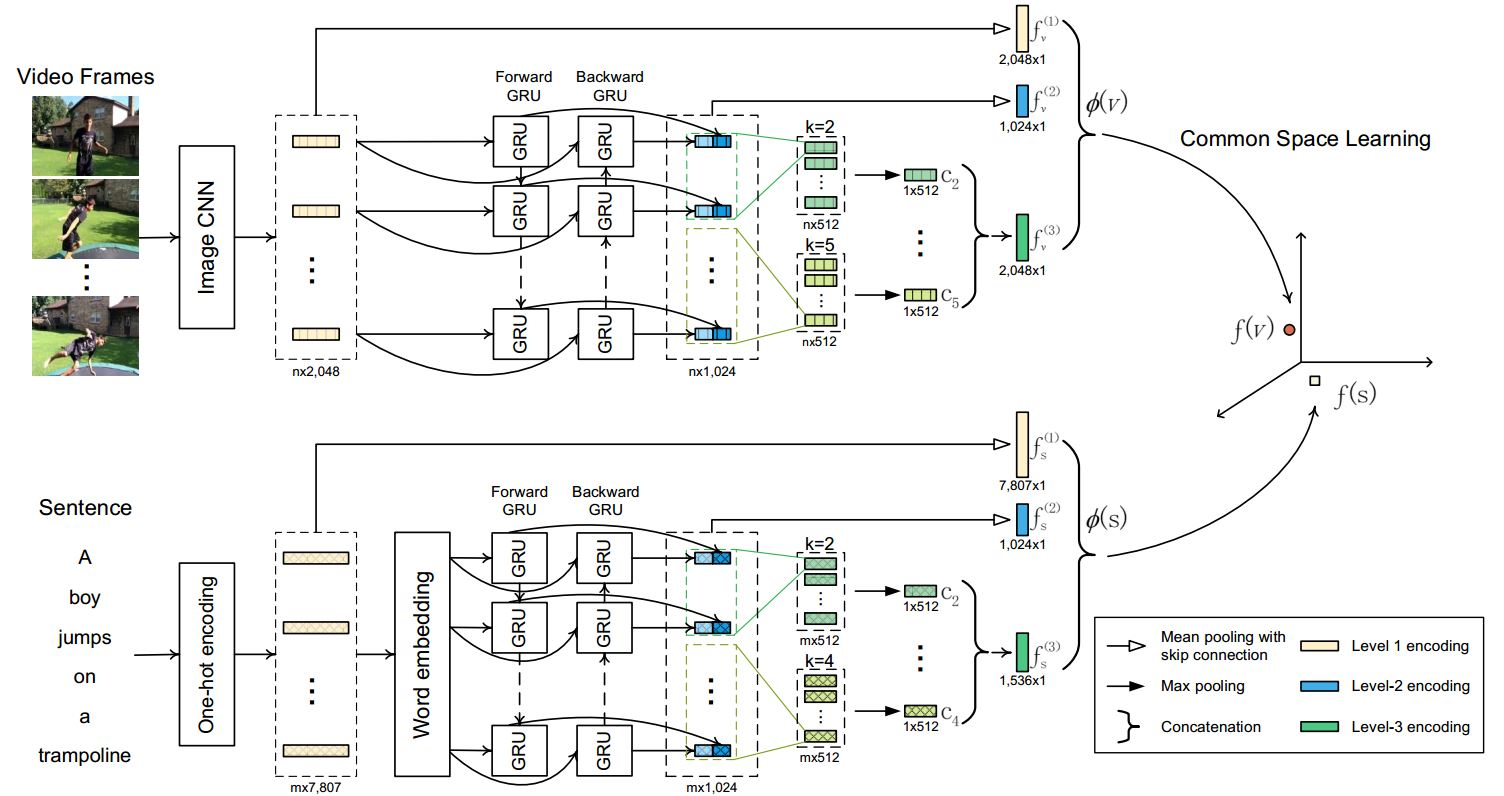
\includegraphics[width=\textwidth]{Resources/dual_encoding.jpg}
\caption{Example of Coordinated Representation learning pipeline\cite{ref_dual_encoding}} \label{fig2}
\end{figure}

\endinput
\chapter{Problem Approach}
\section{Architecture}
After rigor overview of related work, Coordinated Representation techniques were identified as the most prominent direction for our problem. Coordinated Representation approach aims to exploit modality-specific features fully, thus we train each feature modality separately.
% TODO: for our solution? (not problem)

To make the system learn right features in each modality, we map all of them into space where inter-modality similarity can be evaluated but also preserving the intra-modality similarity structure\cite{ref_cross_modal_hash, ref_devise, ref_kiros}. Then we identify loss function, by enforcing ranking function (\ref{eq_rank_loss}) in that space to return high values for mismatches modality pairs and small otherwise. That would be a loss function, which each modality-specific model will be minimizing, thus empowering modality-specific feature learning. You can see visualisation of this idea on Figure \ref{fig2}.

We will focus on integrating recent Word2VisualVec\cite{ref_w2vv} and dual encoding\cite{ref_dual_encoding} models to our more broader and more realistic problem settings. They showed impressive results but were evaluated on more narrow problem. More specifically, they were working with Flickr dataset\cite{ref_flickr} where one image corresponds to 5 descriptive sentences. In our settings we have one article corresponding to multiple images, where all of them having additional metadata such as category, name, description.

This paper is supported by Github repository\footnote{\url{https://github.com/OlehOnyshchak/WikiImageRecommendation}} with all experiments

\section{Methodology}
\subsection{Methodological Approach}
The hypothesis under test is: "it is possible to implement a model to recommend relevant Commons\cite{ref_wiki_commons} images for a specific Wikipedia article using multimodal learning techniques" and implies Quantitative research. It is aiming to discover whether state-of-the-art techniques of multimodal representation learning can solve this specific problem for Wikipedia with not worse precision. 

\subsection{Methods of Data Collection}
Existing Wikipedia data will be used to conduct the research. More specifically, we will use a collection of featured articles\footnote{\url{https://en.wikipedia.org/wiki/Wikipedia:Featured_articles}}, where each page went through thorough manual review procedure by the Wikipedia community and represent the best Wikipedia can offer. Thus it is theoretically the best possible quality for machine learning algorithms.

\subsection{Methods of Analysis}
We will select candidate algorithms by analyzing recent literature surveys of a corresponding domain, and choosing the most prominent state-of-the-art approaches described there. We will also check the most cited approaches to solve a similar problem. In that way, we can ensure that all state-of-the-art methods existing in that field would be reviewed and then the most applicable would be adequately tested.
\endinput
\chapter{Data}
\section{Overview}
All data is publicly available on Wikipedia. Specifically, we have more than 35 million Wikipedia pages with a fair amount of them enriched with images. We also have Commons image dataset\cite{ref_wiki_commons}, containing more than 55 million images\footnote{\url{https://en.wikipedia.org/wiki/Wikimedia_Commons}}. That is the real-world data, where ultimately the solution should be applied.

But for initial problem research we would only use a reliable subset of above specified data for training. In particular, Wikipedia has a notion of featured articles\footnote{\url{https://en.wikipedia.org/wiki/Wikipedia:Featured_articles}}, which are the best articles with qualitative text and a lot of supporting visualization. In other words, it is a high quality dataset of more than 5000 articles, each of which has multiple associated images, which was manually created. Although, it still requires proper preprocessing and cleaning before using.

Particularly, by text we mean the entire article textual content cleared from Wikipedia formatting along with some extra metadata such as categories or title. Images also collected with additional metadata such as filenames or descriptions.

\section{Structure}
\subsection{High-Level Structure}
\begin{lstlisting}[language=json,firstnumber=1]
    .
    +-- page1  
    |   +-- text.json  
    |   +-- img  
    |       +-- meta.json
    +-- page2  
    |   +-- text.json  
    |   +-- img  
    |       +-- meta.json
    :  
    +-- pageN  
    |   +-- text.json  
    |   +-- img  
    |       +-- meta.json
\end{lstlisting}

where:
\begin{itemize}
    \item[$\ast$] pageN - is the title of N-th Wikipedia page and contains all information about the page
    \item[$\ast$] text.json - text of the page saved as JSON. Please refer to the details of JSON schema below.
    \item[$\ast$] meta.json- a collection of all images of the page. Please refer to the detals o of JSON schema below.
    \item[$\ast$] imageN - is the N-th image of an article, saved in `jpg` format where width of each image is set to 600px. Name of the image is md5 hashcode of original image title. 
\end{itemize}

\subsection{text.json Schema}
\begin{lstlisting}[language=json,firstnumber=1]
{
  "title": "Naval Battle of Guadalcanal",
  "id": 405411,
  "url": "https://en.wikipedia.org/wiki/Naval_Battle_of_Guadalcanal",
  "text": "The Naval Battle of Guadalcanal, sometimes referred to.. ",
 }
\end{lstlisting}

where:

\begin{itemize}
    \item[$\ast$] title - page title
    \item[$\ast$] id - unique page id
    \item[$\ast$] url - url of a page on Wikipedia
    \item[$\ast$] text - text content of the article escaped from Wikipedia formatting
\end{itemize}

\subsection{meta.json Schema}

\begin{lstlisting}[language=json,firstnumber=1]
{
  "img_meta": [
    {
      "filename": "d681a3776d93663fc2788e7e469b27d7.jpg",
      "title": "Metallica Damaged Justice Tour.jpg",
      "description": "Metallica en concert",
      "url": "https://en.wikipedia.org/wiki/File%3AMetallica_Damaged_Justice_Tour.jpg",
      "features": [123.23, 10.21, ..., 24.17],
     },
   ]
}
\end{lstlisting}

where:
\begin{itemize}
    \item[*] filename - unique image id, md5 hashcode of original image title
    \item[*] title - image title retrieved from Commons, if applicable
    \item[*] url - url of an image on Wikipedia
    \item[*] features - output of 5-th convolutional layer of ResNet152 trained on ImageNet dataset. Features taken from original images downloaded in `jpeg` format with fixed width of 600px. Practically, it is a list of floats with len = 2048.
\end{itemize}

Please note that some images are not embedded on Wikipedia page from Commons, thus we can only download them in original type \& size. If you want to use those as well, those images should be properly processed later. Each such image can be identified by suffix `.ORIGINAL` in a `filename` and absence of key `features`. Raw images are available in complete version of dataset\footnote{\url{https://drive.google.com/file/d/1l0Oyv2Y6LmPGN3lP9MB6i8WWCinqkYPk/view?usp=sharing}}

\section{Resources}
\begin{itemize}
    \item[*] complete dataset which includes raw images is available from Google Drive \footnotemark[\value{footnote}]
    \item[*] processed dataset is publicly available from Kaggle\footnote{\url{https://www.kaggle.com/jacksoncrow/extended-wikipedia-multimodal-dataset}}
    \item[*] data was collected by fetching featured articles text \& image content with pywikibot library\footnote{\url{https://pypi.org/project/pywikibot/}}
    \item[*] collection script is available on GitHub\footnote{\url{https://github.com/OlehOnyshchak/WikiImageRecommendation/blob/master/article_reader/reader.py}}
\end{itemize}

\endinput 
\chapter{Experiments}

\endinput
\chapter{Conclusions}

\endinput

%----------------------------------------------------------------------------------------
%	THESIS CONTENT - APPENDICES
%----------------------------------------------------------------------------------------

\appendix % Cue to tell LaTeX that the following "chapters" are Appendices

% Include the appendices of the thesis as separate files from the Appendices folder
% Uncomment the lines as you write the Appendices


\chapter{Code}

\section{Pseudocode}

Something on the topic



\endinput
%\include{Appendices/AppendixB}
%\include{Appendices/AppendixC}

%----------------------------------------------------------------------------------------
%	BIBLIOGRAPHY
%----------------------------------------------------------------------------------------


\printbibliography[heading=bibintoc]

%----------------------------------------------------------------------------------------

\end{document}  
